\documentclass{article}
\usepackage{graphicx}
\usepackage{subcaption}
\usepackage{float}
\usepackage{amsmath}
\usepackage{hyperref}

\title{Just-In-Time Software Defect Prediction}
\author{Ali M, Yifei Gong, Yunhua Zhao}
\date{\today}
\begin{document}
\maketitle

\section{Introduction}
Software plays a more and more important role in our real life, a small problem in a software may cause a huge loss,like one of the biggest American market makers for stocks Knight struggled to stay afloat after a software bug triggered a \$440 million loss in just 30 minutes. The primary objective of software quality assurance activities is to reduce the number of defects in software products. Software defect prediction has been an active research area. \\
The defect is found earlier, the cost is less, also now it is a challenging problem considering the limitation of budget and time allocation for such activities~\cite{wan2018perceptions}. Just-in-time software defect prediction(JIT-SDP) extracts features from code changes(eg.codes from a git commit), feed these features to a model then to predict if new code changes are buggy or clean. JIT-SDP predict defects during the code change state, when the knowledge is still fresh to the developers, which help to save the debug time. Figure 1 is an example of buggy commit in OPENSTACK ~\ref{example}, it includes commit id, commit author, commit date, commit message and commit diffs, which describe a defective code submit. 
\begin{figure}[H]
	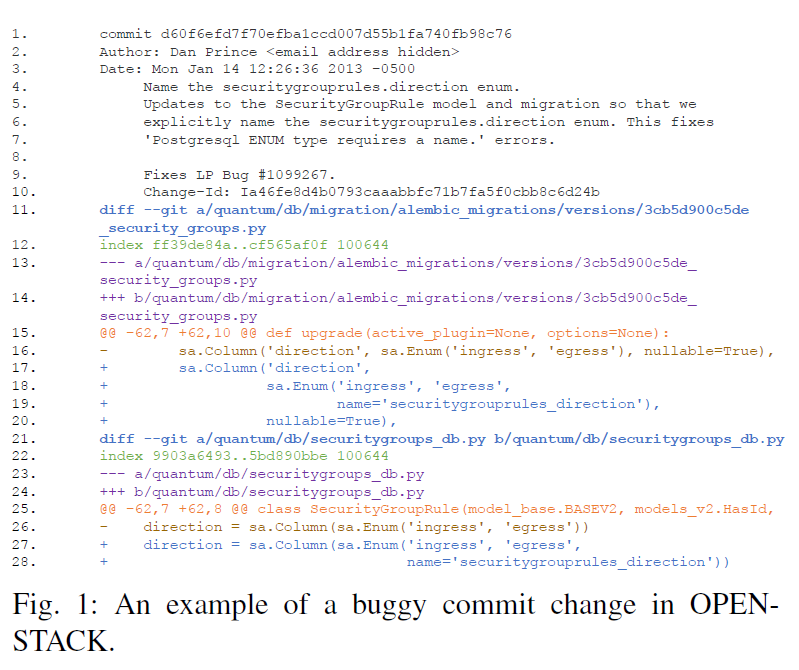
\includegraphics[width=8cm]{1}
	\label{fig:example}
	\centering
\end{figure}


\section{Each team member’s role and contribution}
Our team wants to do experiments and compare to Hoang's paper's result~\cite{hoang2019deepjit}, we will try some simple models and dnn.\\
\begin{itemize}
	\item Dataset exploration: Yifei 
	\item Class balance: Ali
	\item Feature pre-preprocessing: Yunhua
	\item Model build, logistic regression plus dnn: Ali
	\item Model build, random forest tree plus dnn: Yifei
	\item Model build, Bayern Network plus dnn: Yunhua
	\item Evaluation: all of the team will report F1, accuracy auc, recall and precision
	\item Mode comparison: all of the team
	\item Report: All of us need to write their parts report.
\end{itemize}
\section{Enumerate the CSCI 740 related topics (questions and solution approaches) each individual will contribute
	to the project}
\begin{itemize}
	\item Dataset exploration: Yifei\\
	Will plot figures to show the data sets, also calculate the mean, max, min and check if there is na or empty values, and how the correlation of the data set features.
	\item Class balance: Ali  \\
	Try different methods, oversampling(SMOTE) and undersampling methods.
	\item Feature pre-preprocessing: Yunhua  \\
	Check the relationships among features, remove some correlated features, rank them and select features
	\item Model build, tune parameters and visualization, logistic regression plus dnn: Ali
	\item Model build, tune parameters and visualization, random forest tree plus dnn: Yifei
	\item Model build, tune parameters and visualization, Bayern Network plus dnn: Yunhua
	\item Evaluation: all of us will report G-mean, F1, accuracy auc, recall and precision \\
	Will print the results, also plot ROC curve and confusion matrics
	\item Mode comparison: together \\
	Compare our result with Hoang's result~\cite{hoang2019deepjit}, if our results does not win, may try ensemble learning.
	\item Report: All of us need to write their parts report.
\end{itemize}

\section{Describe the dataset}
There are totally 2 data sets: openstack and qt; openstack is for cloud computing and QT is widget toolkit for creating graphical user interfaces. Each of them has 35 features, like lines of modified, developer experience.  
\begin{center}
	\begin{tabular}{ c c c }
		data set & row number & column number \\ 
		\hline
		qt & 25150 & 35 \\ 
		openstack & 26854 & 35 \\  
		\hline
	\end{tabular}
\end{center}

\section{Provide a timeline for the project}
\begin{center}
	\begin{tabular}{ c c  }
		week & work \\ 
		\hline
		04/09/2021-04/16/2021 & data exploration, class balance, pre-processing \\ 
		04/16/2021-04/23/2021 & model build and tune \\  
		04/23/2021-04/30/2021 & evaluation and model comparison \\
		04/30/2021-05/06/2021 & team members result sharing and discussion   \\
		05/06/2021-05/13/2021 & write report  \\ 
		05/13/2021-05/20/2021 & modify report and presentation preparation  \\
		\hline
	\end{tabular}
\end{center}

\section{Describe what you plan to demo on the final exam date and other deliverables}
\begin{itemize}
	\item our data visualization 
	\item our data pre-processing results(store to a file and visualize)
	\item model tuned parameters
	\item evaluation results: F1, accuracy, auc, G-mean
	\item Comparison result with Hoang's paper~\cite{hoang2019deepjit}
\end{itemize}

\section{Describe your plan to evaluate the project.}
We will use the methods studied from this class to these popular dataset in JIT-SDP, then compare to the well-known papers' results, maybe we can make an improvement and find some new angle in this erea.















\medskip

\bibliographystyle{unsrt}
\bibliography{ref}

























































\end{document}